%----------------------------------------------------------------------------------------
%
% A LaTeX-template for 1DV510. Modified and translated by Björn Lindenberg at LNU.
% Based on an original master thesis template created by Marcus Wilhelmsson at LNU.
%
%----------------------------------------------------------------------------------------

% Settings and document configuration

\documentclass[a4paper,12pt]{article} 
\usepackage[T1]{fontenc} 
\usepackage{times} 
\usepackage[swedish,english]{babel} 
\usepackage[utf8]{inputenc} 
\usepackage{dtk-logos} 
\usepackage{wallpaper} 
\usepackage[absolute]{textpos} 
\usepackage[top=2cm, bottom=2.5cm, left=3cm, right=3cm]{geometry} 
\usepackage[parfill]{parskip} 
\usepackage{csquotes} 
\usepackage{float} 
\usepackage{lipsum} % Used for dummy text. Can be removed.
\usepackage{listings, color}

\lstdefinestyle{Asm}{
  belowcaptionskip=1\baselineskip,
  breaklines=true,
  frame=L,
  xleftmargin=\parindent,
  language=[x86masm]Assembler,
  showstringspaces=false,
  basicstyle=\footnotesize\ttfamily,
  keywordstyle=\bfseries\color{purple!40!black},
  commentstyle=\itshape\color{green!40!black},
  identifierstyle=\color{blue},
  stringstyle=\color{orange},
}

% Fontsizes for section headings.
\usepackage{sectsty} 
\sectionfont{\fontsize{14}{15}\selectfont}
\subsectionfont{\fontsize{12}{15}\selectfont}
\subsubsectionfont{\fontsize{12}{15}\selectfont}

%----------------------------------------------------------------------------------------
%	This part is used for the text box on the title page
%----------------------------------------------------------------------------------------
\newsavebox{\mybox}
\newlength{\mydepth}
\newlength{\myheight}

\newenvironment{sidebar}%
{\begin{lrbox}{\mybox}\begin{minipage}{\textwidth}}%
{\end{minipage}\end{lrbox}%
 \settodepth{\mydepth}{\usebox{\mybox}}%
 \settoheight{\myheight}{\usebox{\mybox}}%
 \addtolength{\myheight}{\mydepth}%
 \noindent\makebox[0pt]{\hspace{-20pt}\rule[-\mydepth]{1pt}{\myheight}}%
 \usebox{\mybox}}

%----------------------------------------------------------------------------------------
%	Title
%----------------------------------------------------------------------------------------
\newcommand\BackgroundPic{
    \put(-2,-3){
    
\includegraphics[keepaspectratio,scale=0.3]{img/lnu_etch.png} % Background image
    }
}
\newcommand\BackgroundPicLogo{
    \put(30,740){
    
\includegraphics[keepaspectratio,scale=0.10]{img/logo.png} % LNU logo
    }
}

\title{
\vspace{-8cm}
\begin{sidebar}
    \vspace{10cm}
    \normalfont \normalsize
    \huge Computer Technology I\\ % Main title
    \vspace{-1.3cm}
\end{sidebar}
\vspace{3cm}
\begin{flushleft}
    \huge Lab. 2 : Subroutines % Subtitle
     \small \\ \emph{}
\end{flushleft}
\null
\vfill
\begin{textblock}{5}(10,13)
\begin{flushright}
\begin{minipage}{\textwidth}
\begin{flushleft} \large
\emph{Author:}\textsc{ Loic GALLAND, Leonardo PEDRO}\\  % Author
\emph{Supervisor:}  \textsc{} \\  % Author
\emph{Semester:} Autumn 2019\\ % Semester
\emph{Area:} Computer Science \\ % Area
\emph{Course code:} 1DT301 % Course
\end{flushleft}
\end{minipage}
\end{flushright}
\end{textblock}
}

\date{} % Empty date command. Use \today inside for today's date.
\author{} % Normally one would use this to define authors. However in this case the title command takes care of everything, so we leave the field empty to get rid of warnings. 

\begin{document}

\pagenumbering{gobble} % Turn off page numbering
\newgeometry{left=5cm}
\AddToShipoutPicture*{\BackgroundPic} % Adds the background image to the title page
\AddToShipoutPicture*{\BackgroundPicLogo} % Adds the logo to the title page
\maketitle % Prints the title
\restoregeometry
\clearpage

\pagenumbering{roman} % Roman page numbering for abstract page


\selectlanguage{english}

\newpage

\pagenumbering{gobble} % Turn off page numbering
\tableofcontents 

\newpage
\pagenumbering{arabic} % Turn on page numbering


\section{Task 1 - }

\textit{Write a program that turns ON and OFF a LED with a push button. The LED will be extinguished
when pressing the button.
The program will use Interrupt. Connect the push buttons to PORT D.
The program should have a main program that runs in a loop and wait for the interrupts. An
interrupt routine is called when the push button is pressed. Each time the button is pressed, the
lamp should switch from ‘OFF’ to ‘ON’, or from ‘ON’ to ‘OFF’.}

\lstset{style=Asm}
\begin{lstlisting}
;>>>>>>>>>>>>>>>>>>>>>>>>>>>>>>>>>>>>>>>>>>>>>>>>>>>>>>>>>>>
; 1DT301, Computer Technology I
; Date: 2019-09-29
; Author:
; Loic GALLAND
; Leonardo PEDRO
;
; Lab number: 3
; Title: How to use interrupts
;
; Hardware: STK600, CPU ATmega2560
;
; Function: Program that when clicking on a switch the LEDs switch from ON to OFF and vice versa. It is using interupts to do it.
;
; Input ports: PORTD
;
; Output ports: PORTB
;
; Subroutines: If applicable.
; Included files: m2560def.inc
;<<<<<<<<<<<<<<<<<<<<<<<<<<<<<<<<<<<<<<<<<<<<<<<<<<<<<<<<<<<
.include "m2560def.inc"

.org 0x00	;Location where the program will start
rjmp start

.org INT0addr	;INT0 interrupt address
rjmp interrupt_0

.org 0x72

start:
.def LIGHT = r21	;Give a name to r21
; Initialize SP, Stack Pointer
ldi r20, HIGH(RAMEND) ; R20 = high part of RAMEND address
out SPH,R20 ; SPH = high part of RAMEND address
ldi R20, low(RAMEND) ; R20 = low part of RAMEND address
out SPL,R20 ; SPL = low part of RAMEND address

ldi r16,0xFF	;Load 0xFF into r16 to initialize PORTB
out DDRB,r16	
ldi r16,0x00	;Load 0x00 into r16 and initialize PORTD
out DDRD,r16

ldi r18, 0xFF	;initiliaze the LEDs (turn them off)
out PORTB, r18

mov LIGHT,r18	;Copy the r18 into "LIGHT"
;Initialised the Interrupts
ldi r16, 0b00000010	;INT0 falling edge
sts EICRA, r16	;Setup internal 

ldi r16, 0b00000001	;INT0 enable, pin 0 of PORT D
out EIMSK, r16
sei	;Global interrupt enable

main:
	out PORTB, LIGHT	;Turn on the LEDs
rjmp main

interrupt_0:
	com LIGHT	;Change the 0s into 1s, to show the lights on
RETI	
\end{lstlisting}
This is the flowchart of the task 1:
\begin{center}
%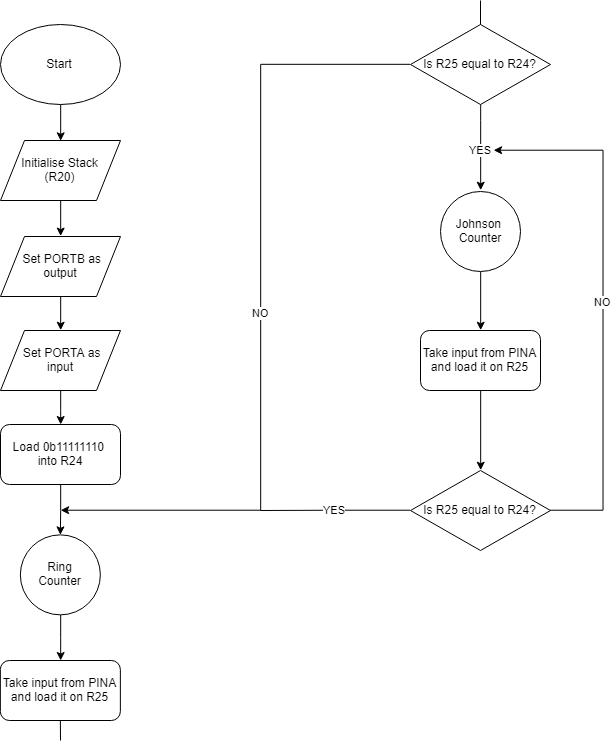
\includegraphics[scale=0.7]{img/Task1.png}
\end{center}
\newpage
\section{Task 2 - Switch – Ringcounter / Johnsoncounter, with interrupt}
\textit{Write a program that by means of a switch can choose to flash 8 LEDs either in the form of a ring
counter or in the form of a Johnson counter. Use the switch SW0 connected to PORTD to switch
between the two counters. Each time the button is pressed, a shift between the two counters
should take place. By using interrupts you’ll swap directly with no delay.}

\lstset{style=Asm}
\begin{lstlisting}
;>>>>>>>>>>>>>>>>>>>>>>>>>>>>>>>>>>>>>>>>>>>>>>>>>>>>>>>>>>>
; 1DT301, Computer Technology I
; Date: 2015-09-03
; Author:
; Student name 1
; Student name 2
;
; Lab number: 3
; Title: How to use interrupts
;
; Hardware: STK600, CPU ATmega2560
;
; Function: Describe the function of the program, so that you can understand it,
; even if you're viewing this in a year from now!
;
; Input ports: Describe the function of used ports, for example on-board switches
; connected to PORTA.
;
; Output ports: Describe the function of used ports, for example on-board LEDs
; connected to PORTB.
;
; Subroutines: If applicable.
; Included files: m2560def.inc
;
; Other information:
;
; Changes in program: (Description and date)
;<<<<<<<<<<<<<<<<<<<<<<<<<<<<<<<<<<<<<<<<<<<<<<<<<<<<<<<<<<<
\end{lstlisting}

This is the flowchart of the task 2:
\newpage
\begin{center}
%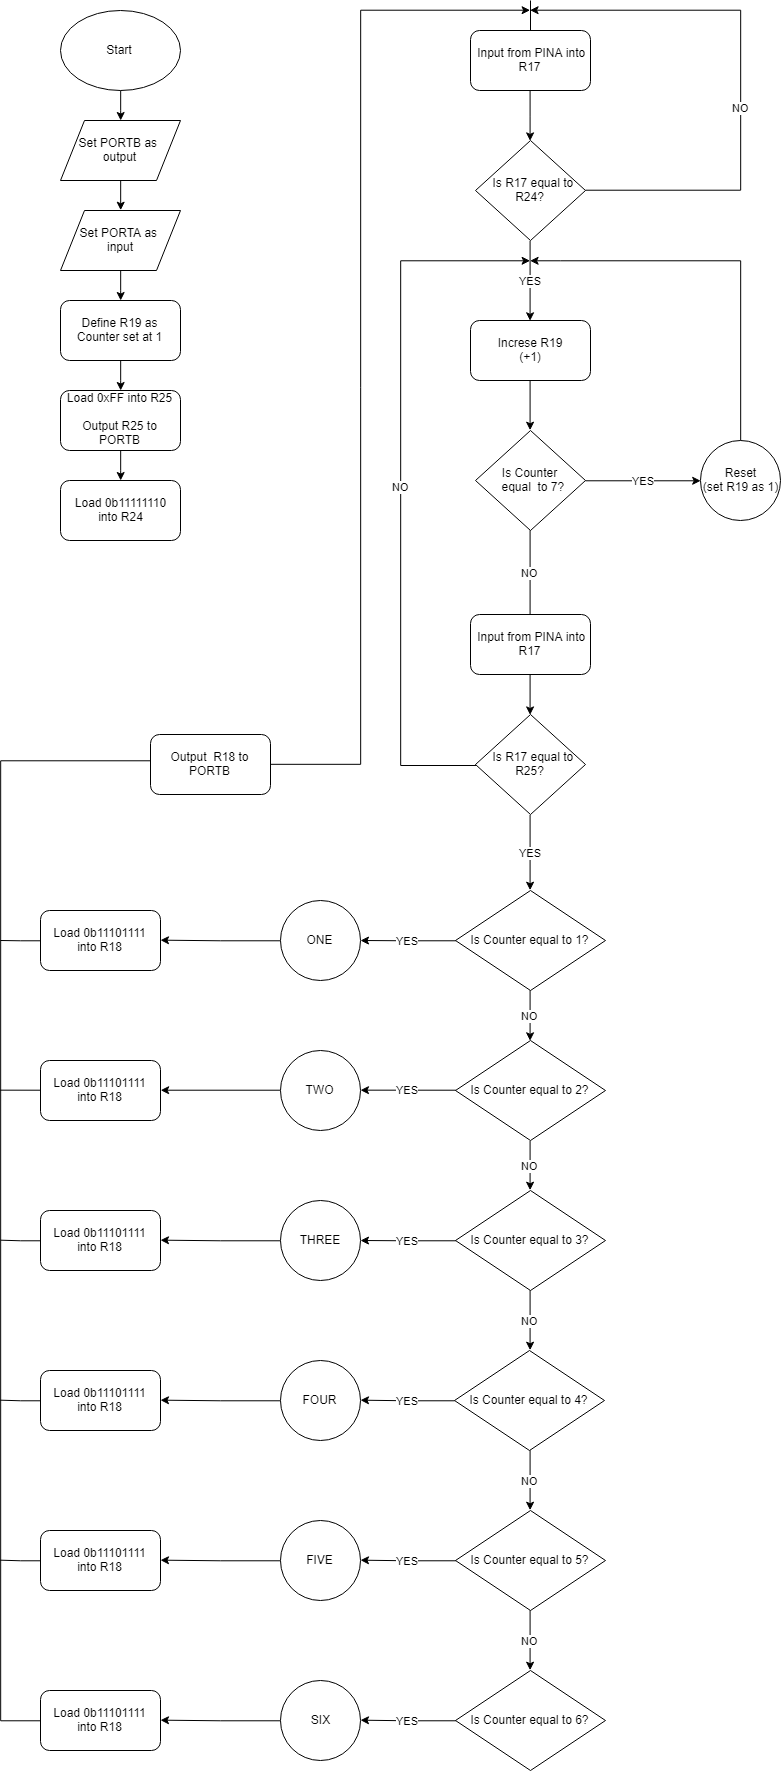
\includegraphics[scale=0.4]{img/Task2.png}
\end{center}

\newpage
\section{Task 3 - Rear lights on a car}
\textit{Program that simulates the rear lights on a car
The 8 LEDs should behave like the rear lights.}

\lstset{style=Asm}
\begin{lstlisting}
;>>>>>>>>>>>>>>>>>>>>>>>>>>>>>>>>>>>>>>>>>>>>>>>>>>>>>>>>>>>
; 1DT301, Computer Technology I
; Date: 2015-09-03
; Author:
; Student name 1
; Student name 2
;
; Lab number: 3
; Title: How to use interrupts
;
; Hardware: STK600, CPU ATmega2560
;
; Function: Describe the function of the program, so that you can understand it,
; even if you're viewing this in a year from now!
;
; Input ports: Describe the function of used ports, for example on-board switches
; connected to PORTA.
;
; Output ports: Describe the function of used ports, for example on-board LEDs
; connected to PORTB.
;
; Subroutines: If applicable.
; Included files: m2560def.inc
;
; Other information:
;
; Changes in program: (Description and date)
;<<<<<<<<<<<<<<<<<<<<<<<<<<<<<<<<<<<<<<<<<<<<<<<<<<<<<<<<<<<
\end{lstlisting}

\newpage
This is the flowchart of the task 3:
\begin{center}
%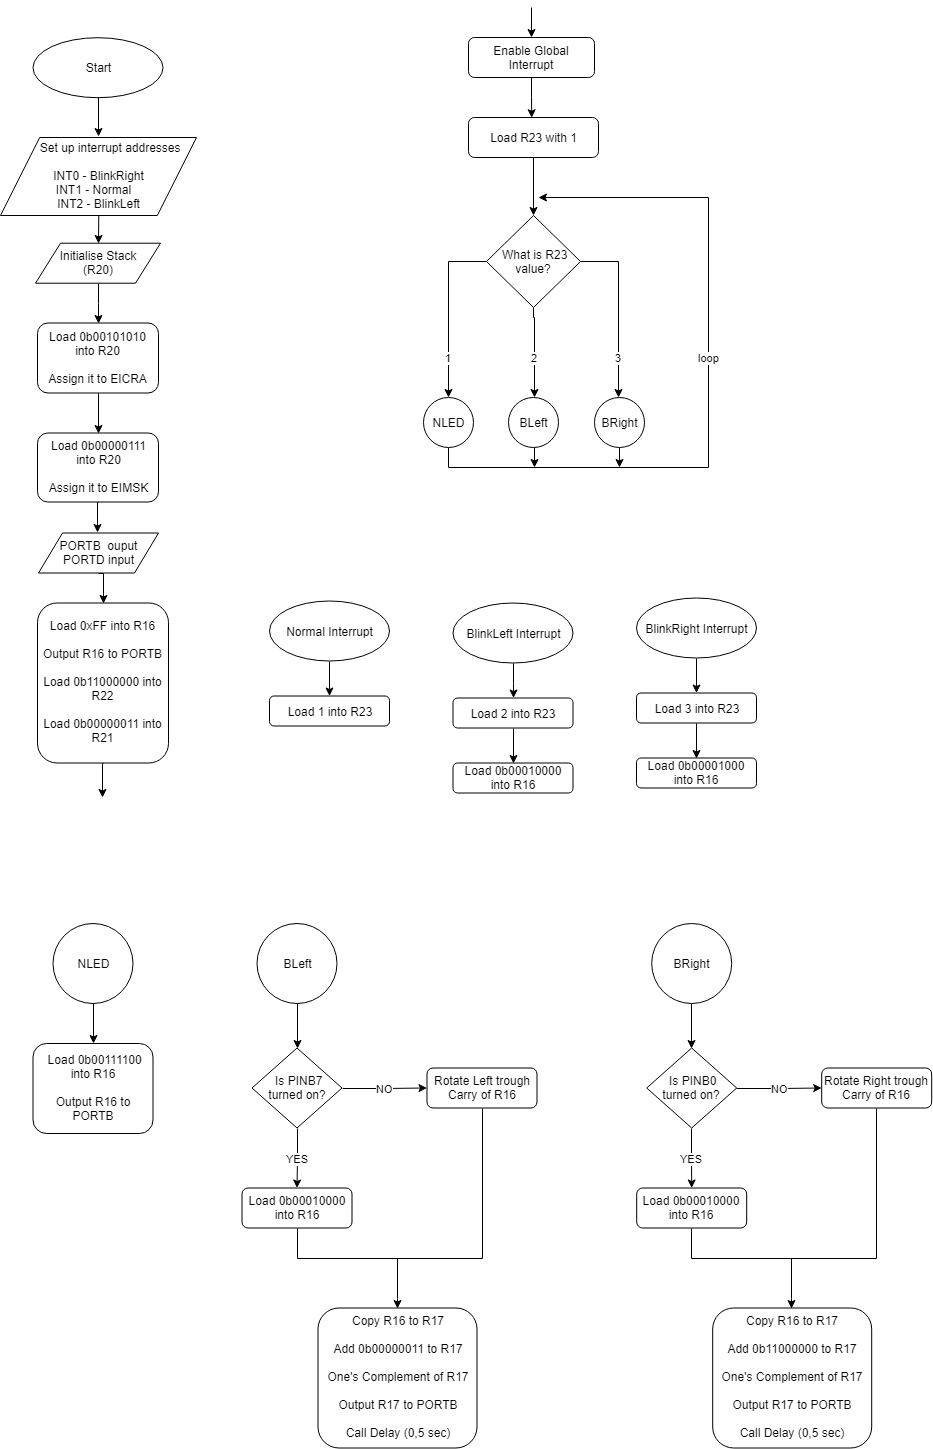
\includegraphics[scale=0.8]{img/TASK3.png}
\end{center}

\newpage
\section{Task 4 - Rear lights on a car, with light for brakes}

\lstset{style=Asm}
\begin{lstlisting}
;>>>>>>>>>>>>>>>>>>>>>>>>>>>>>>>>>>>>>>>>>>>>>>>>>>>>>>>>>>>
; 1DT301, Computer Technology I
; Date: 2015-09-03
; Author:
; Student name 1
; Student name 2
;
; Lab number: 3
; Title: How to use interrupts
;
; Hardware: STK600, CPU ATmega2560
;
; Function: Describe the function of the program, so that you can understand it,
; even if you're viewing this in a year from now!
;
; Input ports: Describe the function of used ports, for example on-board switches
; connected to PORTA.
;
; Output ports: Describe the function of used ports, for example on-board LEDs
; connected to PORTB.
;
; Subroutines: If applicable.
; Included files: m2560def.inc
;
; Other information:
;
; Changes in program: (Description and date)
;<<<<<<<<<<<<<<<<<<<<<<<<<<<<<<<<<<<<<<<<<<<<<<<<<<<<<<<<<<<
\end{lstlisting}

\newpage
This is the flowchart of the task 4:
\begin{center}
%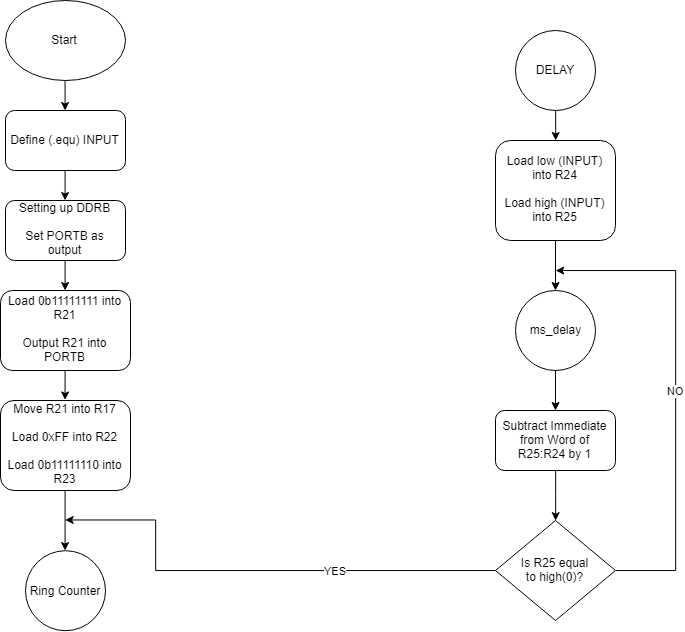
\includegraphics[scale=0.7]{img/Task4.png}
\end{center}
% Prints your bibliography database xxx.bib
\bibliographystyle{IEEEtran}
\bibliography{ref.bib}

\end{document}
